%% ============================================================
%% 分片 23：原文第 9 节「't Hooft And Hecke Operators」（原文 glshort.tex 起于第 6755 行）
%% 由 tools/harvmac2tex.py 从 arXiv 源码（hep-th/0604151v3）自动生成。
%% 只译英文散文；公式、编号、\label、\cite 一律不改。
%% ============================================================

\subsection{'t Hooft 算子与 Hecke 修正}

\label{sec:theck}

先考虑 $W=\Bbb{R}^3$ 上的 Bogomolny 方程，我们把 $\Bbb{R}^3$ 看作 $\Bbb{R}\times\Bbb{C}$，其中 $\Bbb{C}$ 用 $z=x^2+ix^3$ 参数化，$\Bbb{R}$ 用 $y=x^1$ 参数化。我们有 % 式 (9.6)
\setcounter{equation}{5}
\begin{equation}\label{eq:boffo}
\begin{aligned}\star dy&={i\over 2}dz\wedge
d\bar z\\
        \star dz&=-idz\wedge dy\\
        \star d\bar z& = id\bar z\wedge dy.\\\end{aligned}
\end{equation}

把 $F=dz\wedge d\bar z \,F_{z\bar z}+dy\wedge dz
        F_{yz}+dy\wedge d\bar z F_{y\bar z}$ 展开（同样地展开
$D\phi_0=dy D_y\phi_0+dz D_z\phi_0+d\bar z D_{\bar z}\phi_0$），
Bogomolny 方程变为 % 式 (9.7)
\setcounter{equation}{6}
\begin{equation}\label{eq:noffo}
\begin{aligned}F_{z\bar
z}&={i\over 2}D_y\phi_0\\
                    F_{yz}&=iD_z\phi_0\\
                    F_{y\bar z}&=-iD_{\bar z}\phi_0.\\\end{aligned}
\end{equation}

更一般地，取 $W= \Bbb{R}\times C$，其中 $C$ 是黎曼面。用 $z$ 记 $C$ 上的局部复坐标，给 $C$ 配上 Kähler 度量 $h(z,\bar z)|dz|^2$（$h$ 为某正函数），并取 $W$ 上的度量为 $h(z,\bar
z)|dz|^2+dy^2$。\eqref{eq:boffo}\ 与 \eqref{eq:noffo}\ 中的第一式分别变为 % 式 (9.8)
\setcounter{equation}{7}
\begin{equation}\label{eq:jungol}
\begin{aligned}\star dy& ={ih\over 2}\,dz\wedge
d\bar z\\ F_{z\bar z}&={ih\over 2}D_y\phi_0.\end{aligned}
\end{equation}
 其余
方程不变。

复维数为 1 时，$\bar\partial $ 算子没有可积性条件。因此 $G$-丛
$E\to C$ 上的任何联络 $A$ 都给 $E$ 赋予一个全纯结构。我们只需
把 $\bar \partial$ 算子定义为 $\bar D=d\bar z D_{\bar
z}=d\bar z(\partial_{\bar z}+A_{\bar z})$。

\begin{figure}[htbp]
\centering
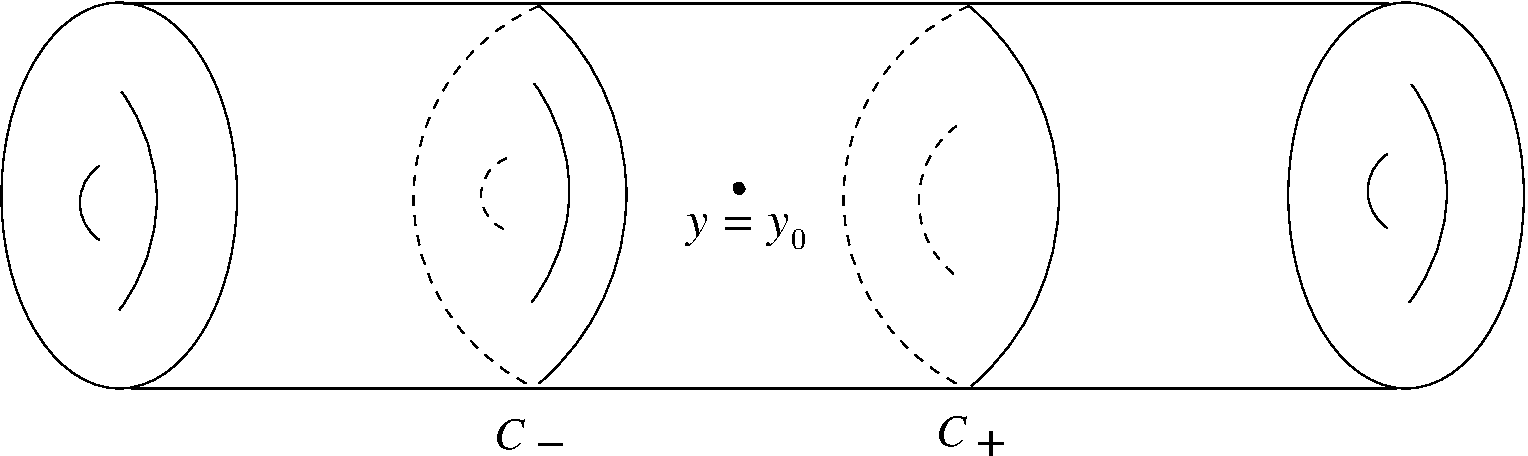
\includegraphics[width=0.75\linewidth]{figures/gla7-2.png}
\caption{在 $G$-丛 $E$ 上 Bogomolny 方程的解中，$E_y$（即 $E$ 到 $\{y\}\times C$ 的限制）的全纯型是常数，除非越过某个 't Hooft 算子的位置。图中画出了位于 $y=y_0$ 的 't Hooft 算子，以及 $y_0$ 左右两侧的 $C_y=\{y\}\times C$ 的一些拷贝，分别记作 $C_-$ 与 $C_+$。（原文 Fig.~13）}
\label{fig:otampo}
\end{figure}

于是，当 $y$ 在 $ \Bbb{R}$ 中变动时，$G$-丛 $E\to  \Bbb{R}\times C$ 上的任何联络 $A$ 都定义了一族全纯 $G$-丛 $E_y\to C$。$E_y$ 就是 $E$ 到 $C_y= \{y\}\times C$ 的限制（\otampo）。现在假设 $A$ 满足 Bogomolny 方程。让我们在规范 $A_y=0$ 中工作。此时 $F_{y\bar z}=\partial_yA_{\bar z}$。因此 \eqref{eq:noffo}\ 中的最后一个方程告诉我们 % 式 (9.9)
\setcounter{equation}{8}
\begin{equation}\label{eq:troffo}
{\partial\over
\partial y}A_{\bar z}=-iD_{\bar z}\phi_0.
\end{equation}

但右端是 $A_{\bar z}$ 在由 $-i\phi_0$ 生成的规范变换下的变化。因此 $E_y$ 的全纯型与 $y$ 无关。（陈述这个论证的另一种方式是注意到 $\partial_y\bar D=-i[\bar D,\phi_0]$，这表明 $\bar D$ 在共轭意义下与 $y$ 无关。）

现在来看看，若在 $\Bbb{R}\times C$ 中的点 $p=y_0\times p_0$ 处加入一个 't Hooft 算子会发生什么。这意味着我们考虑定义在点 $p$ 的补集上、并在 $p$ 附近具有某种类型奇点的丛 $E$ 与联络 $A$，如第~\ref{sec:tophooft}~节所述。

在 $y=y_0$ 之外，上述论证适用，$E_y$ 的全纯型与 $y$ 无关。在 $y=y_0$ 处，由于奇点，丛 $E_y$ 没有定义。越过 $y=y_0$ 时，丛的全纯型可能跳跃。然而，它只能以非常特殊的方式跳跃。若把 $E$ 限制到 $C\backslash p_0$（即 $p_0$ 在 $C$ 中的补集），则上述论证适用，限制后的丛 $E_y$ 的全纯型即使在 $y=y_0$ 处也是常数。所以 $E_y$ 的全纯型可以在 $y=y_0$ 处跳跃，但只能以一种在从 $C$ 中删去点 $p_0$ 后便成为平凡的方式跳跃。

下面我们试图精确描述 $E_y$ 在 $y=y_0$ 处可以如何跳跃。先考虑阿贝尔情形，再考虑非阿贝尔情形。

\par\medskip{\it 阿贝尔情形}

从 $G=U(1)$ 开始。此时 $E$ 是复线丛 ${\cal L}$。把 $y<y_0$ 时的 ${\cal L}_y$ 记为 ${\cal L}_-$，把 $y>y_0$ 时的 ${\cal L}_y$ 记为 ${\cal L}_+$。线丛 ${\cal L}_-$ 与 ${\cal L}_+$ 在点 $p_0\in C$ 的补集上同构。

这意味着线丛 ${\cal L}_+\otimes {\cal L}_-^{-1}$ 在 $p_0$ 之外平凡。于是它有截面 $s$，该截面在 $p_0$ 之外既无零点也无极点；令 $q$ 为其在 $p_0$ 处零点的阶数。则 ${\cal L}_+\otimes {\cal L}_-^{-1}\cong {\cal O}(p_0)^q$。这里照例 ${\cal O}(p_0)$ 是这样一个线丛：其全纯截面是 $p_0$ 之外全纯、在 $p_0$ 处至多有一个单极点的函数。于是 ${\cal L}_+$ 与 ${\cal L}_-$ 的关系为 ${\cal L}_+\cong {\cal L}_-\otimes {\cal O}(p_0)^q$，其中 $q$ 为某个整数。

我们回忆一下，群 $G=U(1)$ 的 't Hooft 算子 $T(m)$ 由整数 $m$ 的选择来分类。（若要指明点 $p_0$，我们把它写成 $T(m;p_0)$。）这提示了一个显然的猜想：$m$ 可能就等于上一段中的整数 $q$。

算子 $T(m)$ 的定义是：在 $p=p_0\times y_0$ 附近，曲率具有奇异行为 % 式 (9.10)
\setcounter{equation}{9}
\begin{equation}\label{eq:formigo}
F\sim
\star d\left({im\over 2}{1\over |\vec x - p|}\right),
\end{equation}
 其中
$|\vec x-p|$ 是 $p$ 到附近点 $\vec x\in
 \Bbb{R}\times C$ 的距离。这意味着，若 $S$ 是如图中那样包围点 $p$ 的小球面，则 $\int_S c_1({\cal L})=m$。因此 't Hooft 算子 $T(m)$ 彼此在拓扑上都是不同的。这个论断（若 $G$ 非阿贝尔则远不成立）将使我们在阿贝尔情形下仅凭拓扑理由就确定 $T(m)$ 的作用。

\begin{figure}[htbp]
\centering
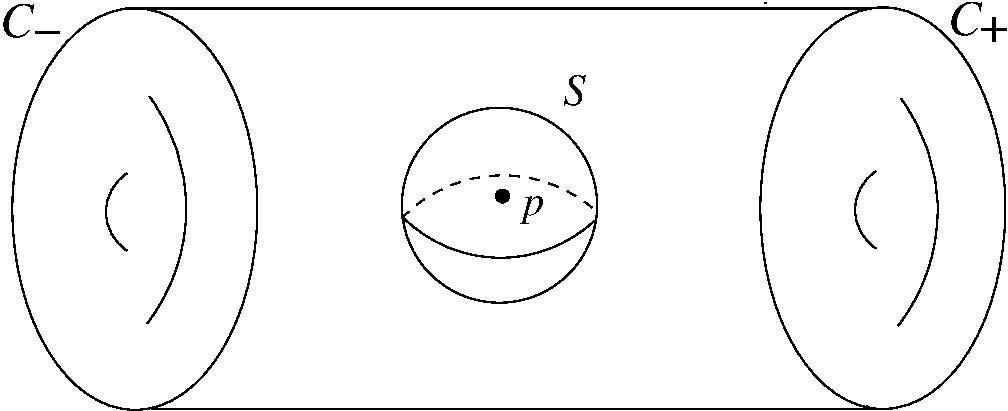
\includegraphics[width=0.75\linewidth]{figures/gla7-3.png}
\caption{二维闭链 $C_-+S$ 与 $C_+$ 之间的一个配边（cobordism），表明同调闭链 $D=C_+-C_--S$ 是一个边界。（原文 Fig.~14）}
\label{fig:notampo}
\end{figure}

 现在取满足 $y_-<y_0<y_+$ 的 $y_\pm$，把 $y_\pm\times C$ 记为 $C_\pm$，于是 ${\cal L}_\pm $ 是 ${\cal L}$ 到 $C_\pm$ 的限制。令 $q_\pm=\int_{C_\pm}c_1({\cal L})$。按 \notampo 中那样显然的定向选择，同调闭链 $D=C_+-C_--S$ 是 $(\Bbb{R}\times C)\backslash p$ 中的一个边界。因此 $0=\int_Dc_1({\cal L})=\int_{C_+}c_1({\cal L})-\int_{C_-}c_1({\cal L})-\int_Sc_1({\cal L})=q_+-m-q_-$。

所以 $q_+=m+q_-$。因此，在 $p_0$ 之外同构的 ${\cal L}_+$ 与 ${\cal L}_-$，其第一 Chern 类相差 $m$。于是 ${\cal L}_+\cong {\cal L}_-\otimes {\cal O}(p_0)^m$。

这样，我们就确定了 $G=U(1)$ 时 't Hooft 算子的作用。't Hooft 算子 $T(m;p_0)$，即在点 $p_0\in C$ 处插入的算子 $T(m)$，通过用 ${\cal O}(p_0)^m$ 扭化来作用。这个结果与 $U(1)$ 的 Hecke 算子的标准定义一致。

我们看到，与第~\ref{sec:lineop}~节的一般论证一致，插入在 $C$ 中不同点处的 't Hooft 算子彼此对易。此外，给定点 $p_0\in C$ 处的 't Hooft 算子构成一个交换群，满足 $T(m;p_0)=T(1;p_0)^m$。

\par\medskip{\it 非阿贝尔情形：$U(N)$}

现在讨论非阿贝尔情形中 't Hooft 算子的作用。先考虑群 $U(N)$。有两件事使这个群易于分析：$U(N)$ 有一个方便的表示，即我们记作 $\VV$ 的 $N$ 维表示；并且 $U(N)$ 是它自己的 Langlands 对偶。

't Hooft 算子的定义依赖于同态 $\rho:U(1)\to U(N)$ 的选择（模共轭）。最一般的这种同态把 $\exp({i\alpha})\in U(1)$ 映为对角矩阵 ${\rm
diag}(\exp({im_1\alpha}),\exp({im_2\alpha}),\dots,
\exp({im_N\alpha}))$，其中整数 $N$ 元组
$^L\negthinspace w=(m_1,m_2,\dots,m_N)$ 在置换意义下唯一。（我们把这个量记作 $^L\negthinspace w$，因为在一般情形下它将是 Langlands 对偶群 $^L\negthinspace G$ 的一个权。）我们通常把 $m_i$ 排序使 $m_1\geq
m_2\geq \dots\geq m_N$。在 Lie 代数层面，$\rho$ 把 $1\in \frak{u}(1)$ 映为对角矩阵
% 式 (9.11)
\setcounter{equation}{10}
\begin{equation}\label{eq:morphy}
\left(\begin{matrix}m_1& & & \dots & \\
                                    &m_2& & \dots & \\
                          & & m_3 &\dots & \\
                & & \vdots & \dots& \\
            & & & & m_N\\\end{matrix}\right).
\end{equation}

相应的 't Hooft 算子 $T(^L\negthinspace w)$ 的定义是：在点 $p\in  \Bbb{R}\times C$ 附近，规范场具有把基本 $U(1)$ 奇点通过该嵌入映入 $U(N)$ 所得的奇点。例如，$p$ 附近曲率的奇异部分为对角的
% 式 (9.12)
\setcounter{equation}{11}
\begin{equation}\label{eq:orphy}
F\sim \star d\left({i\over 2}{1\over |\vec x -
p|}\right) \left(\begin{matrix}m_1& & & \dots & \\
                                    & m_2& & \dots & \\
                          & & m_3 &\dots & \\
                & & \vdots & \dots& \\
            & & & & m_N\\\end{matrix}\right).
\end{equation}

在 $p$ 附近，Bogomolny 方程约化为 $U(N)$ 的某个极大环面 ${\cal T}=U(1)^N$ 中的方程。（从全纯观点看，更自然的做法是考虑相应的、约化到规范群复化中的复化极大环面的方程，即约化到 $U(N)_{\Bbb{C}}=GL(N,\Bbb{C})$。）与方程约化到极大环面相应，丛 $E_y$ 在 $p_0\times y \in C_y$ 附近分裂为线丛之和 ${\cal L}_1\oplus {\cal L}_2\oplus\dots \oplus {\cal L}_N$（它们每一个当然都在 $p$ 附近平凡）。't Hooft 算子对 ${\cal L}_i$ 的作用恰与阿贝尔情形相同，即 ${\cal L}_i\to {\cal L}_i\otimes {\cal O}(p_0)^{m_i}$。

这样，我们就得到了 't Hooft 算子 $T(^L\negthinspace w)$ 在丛 $E$ 上如何作用的描述。相对于 $E$ 在 $p$ 附近作为 $\oplus_{i=1}^N{\cal L}_i$ 的某个分解，它通过 ${\cal L}_i\to {\cal L}_i\otimes {\cal O}(p_0)^{m_i}$ 作用。这与 $U(N)$ 的 Hecke 算子作用的通常数学描述一致。这就是 't Hooft 算子与 Hecke 算子之间的基本联系。

在第~\ref{sec:spaceheck}~节 与 第~\ref{sec:affgrass}~节中，我们将讨论 $E$ 的局部分解 $E=\oplus_{i=1}^N{\cal L}_i$ 中包含何种数据，以及其中多少数据与 't Hooft 算子的作用相关。这个问题的通常答案涉及所谓仿射 Grassmann 流形，我们将在第~\ref{sec:affgrass}~节中简要描述。

\par\medskip{\it 若干例子}

一般地，正如我们从第~\ref{sec:tophooft}~节所知，Langlands 对偶群 $^L\negthinspace G$ 的表示自然地对应于 $G$ 的 't Hooft 算子。最高权为 $^L\negthinspace w$ 的表示 $R(^L\negthinspace w)$ 对应于一个 't Hooft 算子，我们把它写作 $T(R(^L\negthinspace w))$，或简记为 $T(^L\negthinspace w)$。在当前的讨论中，$^L\negthinspace G=G=U(N)$。

例如，$U(N)$ 的基本 $N$ 维表示 $\VV$ 在我们约定 $m_1\geq m_2\geq \dots\geq m_N$ 下的最高权为 $^L\negthinspace w(1)=(1,0,0,\dots,0)$，它对应于 't Hooft 算子 $T(^L\negthinspace w(1))$，或简记为 $T_{(1)}$。对 $k=1,\dots,N$，第 $k$ 个反对称张量表示 $\wedge^k\VV$ 的最高权为 % 式 (9.13)
\setcounter{equation}{12}
\begin{equation}\label{eq:nyto}
^L\negthinspace
w(k)=(\overbrace{1,1,\dots,1}^{\text {$k$ times}},0,\dots,0)
\end{equation}
 并
对应于 't Hooft 算子 $T_{(k)}$。

表示 $\wedge^N\VV$ 是一维的；它是 $g\in U(N)$ 通过乘以 $\det(g)$ 作用的表示。它可以提升到任意整数幂 $u$（正或负），得到 $g$ 通过 $(\det(g))^u$ 作用的表示。这个表示我们记作 $(\wedge^N\VV)^u$，它对应于权 $^L\negthinspace w=(u,u,\dots,u)$。对应于 $\wedge^N\VV$ 的 't Hooft/Hecke 算子 $T_{(N)}$ 简单地通过 $E\to E\otimes {\cal O}(p_0)$ 作用（如同阿贝尔情形），并且显然是可逆的。它的 $u$ 次幂对应于表示 $(\wedge^N\VV)^u$。而 $k<N$ 的 $T_{(k)}$ 不可逆。

$U(N)$ 的中心元素 $\exp(i\alpha)$ 在表示 $\wedge^k\VV$ 上通过乘以 $\exp(ik\alpha)$ 作用。更一般地，它在最高权为 $^L\negthinspace w=(m_1,m_2,\dots,m_N)$ 的任何表示上通过乘以 $\exp(i\alpha\sum_{i=1}^Nm_i)$ 作用。这个陈述的一个特例是：$U(N)$ 的中心平凡作用当且仅当 % 式 (9.14)
\setcounter{equation}{13}
\begin{equation}\label{eq:hoty}
\sum_im_i=0.
\end{equation}
 $S$-对偶，正如我们在第~\ref{sec:electricbranes}~节讨论过的，把 $^L\negthinspace G$ 的中心在表示 $^L\negthinspace R$ 上的作用，映为相应的 't Hooft 算子 $T(^L\negthinspace R)$ 对 $G$-丛拓扑的作用。确实，由于 $T(^L\negthinspace w)$ 局部把 $\oplus_i{\cal L}_i$ 映为 $\oplus_i\left({\cal L}_i\otimes {\cal O}(p_0)^{m_i}\right)$，它把 $c_1(E)$ 改变为 % [WARN] 公式 \eqn\eqref{eq:yorgo} 无编号或重复
\begin{equation*}
\tag*{(9.15)}
c_1(E)\to c_1(E)+\sum_im_i,
\end{equation*}
 于是
$E$ 的拓扑不变当且仅当 $\sum_im_i=0$。

由 $S$-对偶，我们预期 $G$ 的 't Hooft 算子构成一个交换代数，同构于 $^L\negthinspace G$ 的表示环。（事实上，正如我们在第~\ref{sec:lineop}~节讨论过的，'t Hooft 算子的对易性可由四维拓扑场论的更一般考虑得出，而不必借助 $S$-对偶。）我们将在第~\ref{sec:kahstr}~节 从 Bogomolny 方程的角度考察这一点。$U(N)$ 的表示环由表示 $\wedge ^k\VV,\,k=1,\dots,N$ 连同 $(\wedge^N\VV)^{-1}$ 自由生成。相应地，$U(N)$ 的 't Hooft 算子构成的交换代数由 $T_{(k)}$ 连同 $T_{(N)}^{-1}$ 自由生成。在几何 Langlands 纲领的数学文献中，这些生成元通常被取作 $U(N)$ 的基本 Hecke 运算。

\par\medskip{\it 其他群的 't Hooft/Hecke 算子}

把这一切推广到任意紧规范群 $G$ 相当直接。为使讨论相对简单，我们取 $G$ 的一个表示 $R$，并考虑取在表示 $R$ 中的 $G$-丛 $E_R$。（于是，若 $E$ 表示主 $G$-丛，则 $E_R=E\times_G R$。）取 $G$ 的一个极大环面 ${\cal T}$，用 $w$ 记 $G$ 的一个权，即特征 $w:{\cal T}\to U(1)$。令 $R=\oplus_wR_w$ 为 $R$ 按权空间 $R_w$ 的分解（其中除有限多个外，这些权空间都为零）。

$G$ 的 't Hooft 算子由支配余权 $^L\negthinspace w:U(1)\to {\cal T}$ 分类，它是对偶群 $^L\negthinspace G$ 的某个表示 $^L\negthinspace R$ 的最高权。$w:{\cal T}\to U(1)$ 与 $ ^L\negthinspace w:U(1)\to {\cal T}$ 的复合是一个同态 $w\circ{}^L\negthinspace w:U(1)\to U(1)$，其形式为 $\exp(i\alpha)\to \exp(i\langle ^L\negthinspace w,w\rangle\alpha)$，其中 $\langle ^L\negthinspace w,w\rangle$ 是某个整数。

对 $G_{\Bbb{C}}$ 的任一复化极大环面 ${\cal T}_{\Bbb{C}}$ 的选择，$E_R$ 在 $p_0\in C$ 处的纤维都有按权空间的分解 $E_R|_{p_0}=\oplus_w E_{R,w}|_{p_0}$。若把 ${\cal T}$ 延拓为 $p_0$ 附近全纯变化的极大环面族，我们就得到 $E_R$ 相应的、按确定权分解为子丛的局部分解：$E_R=\oplus_w {E}_{R,w}$。通过在 $p_0$ 附近求解 Bogomolny 方程，并考虑到奇点的阿贝尔性质，我们发现：相对于这样的某种分解，$T(^L\negthinspace w)$ 通过 ${E}_{R,w}\to {E}_{R,w}\otimes {\cal O}(p_0)^{\langle ^L\negthinspace w,w\rangle}$ 作用。

我们将对 $G=SU(N)$、$^L\negthinspace G=PSU(N)=SU(N)/\Bbb{Z}_N$ 的情形，以及互反的情形 $G=PSU(N)$、$^L\negthinspace G=SU(N)$ 作更具体的说明。

同态 $\rho:U(1)\to G=SU(N)$ 取与 $U(N)$ 情形相同的形式，即 $\exp(i\alpha)\to{\rm diag}(\exp({im_1\alpha}),\exp({im_2\alpha}),\dots,\exp(im_N\alpha))$，只不过现在必须要求 $\sum_im_i=0$，如 \eqref{eq:hoty} 那样。相应的 't Hooft 算子 $T(^L\negthinspace w)$ 对 $SU(N)$ 丛 $E$ 的作用与前面一样：相对于 $p$ 附近的某个分解 $E=\oplus_{i=1}^N{\cal L}_i$，有 ${\cal L}_i\to {\cal L}_i\otimes {\cal O}(p_0)^{m_i}$。

按我们通常的排序 $m_1\geq m_2\geq\dots\geq m_N$，$N$ 元组 $^L\negthinspace w=(m_1,m_2,\dots,m_N)$ 是 $SU(N)$ 的单根 $e_1=(1,-1,0,\dots,0)$、$e_2=(0,1,-1,0,\dots,0),\dots ,e_{N-1}=(0,0,\dots,0,1,-1)$ 的正整数组合。因此它是伴随群 $PSU(N)$ 的某个表示的最高权，而在此情形下 $PSU(N)$ 当然与 $^L\negthinspace G$ 重合。

现在讨论 $G=PSU(N)$、从而 $^L\negthinspace G=SU(N)$ 的情形。同态 $\rho:U(1)\to PSU(N)$ 可以提升为从 $U(1)$ 的 $N$ 重覆盖到 $SU(N)$ 的同态。这样的同态取形式 $\exp(i\alpha)\to{\rm diag}(\exp(im_1\alpha),\exp(im_2\alpha),\dots,\exp(im_N\alpha))$，但 $m_i$ 不是整数；它们取值于 ${1\over N}\Bbb{Z}$，而差 $m_i-m_j$ 为整数。这样按 $m_1\geq m_2\geq \dots\geq m_N$ 排序的 $N$ 元组 $^L\negthinspace w=(m_1,m_2,\dots,m_N)$ 是 $^L\negthinspace G=SU(N)$ 的支配权。它对应于 $SU(N)$ 的一个表示 $^L\negthinspace R$，以及 $G=PSU(N)$ 的 't Hooft 算子 $T(^L\negthinspace R)$。使 $SU(N)$ 的中心非平凡作用的那些表示 $^L\negthinspace R$（从而 $T(^L\negthinspace R)$ 改变 $PSU(N)$-丛拓扑的那些表示），正是使 $m_i$ 为非整数的那些表示。

设 $E$ 是主 $PSU(N)$ 丛。由于 $PSU(N)$ 没有与 $SU(N)$ 的 $N$ 维表示 $\VV$ 相对应的 $N$ 维表示，我们无法从 $E$ 得到秩 $N$ 的复向量丛 $E_\VV$。然而，$E_\VV$ 作为扭化向量丛（twisted vector bundle）是存在的；这个概念我们在第~\ref{sec:comptwop}~节简要解释过。把 $E_\VV$ 提升为普通向量丛的阻碍是在第~\ref{sec:reviewthis}~节引入的特征类 $\xi(E)$。取定一族极大环面后，$E_\VV$ 有局部分解 $E_\VV=\oplus_{i=1}^N{\cal L}_i$，其中 ${\cal L}_i$ 是扭化线丛（它们都以相同方式扭化，因为把 $E_\VV$ 提升为向量丛的阻碍是中心的）。

't Hooft/Hecke 算子相对于某种这样的分解，按熟悉的方式 ${\cal L}_i\to{\cal L}_i\otimes {\cal O}(p_0)^{m_i}$ 作用。但现在 $m_i$ 可能不是整数。我们把 ${\cal O}(p_0)^{1/N}$ 定义为一个扭化线丛，并对任意整数 $m$ 把 ${\cal O}(p_0)^{m/N}$ 定义为 ${\cal O}(p_0)^{1/N}$ 的 $m$ 次幂。特别地，${\cal O}(p_0)^{1/N}$ 的 $N$ 次幂是普通线丛 ${\cal O}(p_0)$。由于差 $m_i-m_j$ 是整数，扭化线丛 ${\cal O}(p_o)^{m_i}$ 都以相同方式扭化，而 't Hooft/Hecke 算子通过 ${\cal L}_i\to {\cal L}_i\otimes {\cal O}(p_0)^{m_i}$ 的作用保持所有 ${\cal L}_i$ 具有相同扭化这一事实。

当然，我们可以避开谈论扭化丛：取 $PSU(N)$ 的一个表示 $R$，把 't Hooft 算子作用于普通向量丛 $E_R=E\times_{PSU(N)}R$。例如取 $N=2$，于是 $PSU(2)$ 成为 $SO(3)$。秩 2 扭化丛 $E_\VV$ 有局部分解 ${\cal L}\oplus {\cal L}^{-1}$，其中 ${\cal L}$ 是扭化线丛。若取 $R$ 为 $SO(3)$ 的伴随表示，则相应的伴随丛 $E_R$ 是 ${\rm Sym}^2(E_\VV)$（$E_\VV\otimes E_\VV$ 的对称部分），或 ${\cal L}^2\oplus {\cal O}\oplus {\cal L}^{-2}$，其中 ${\cal L}^2$ 是普通线丛。变换 ${\cal L}\to {\cal L}\otimes {\cal O}(p_0)^{1/2}$ 通过 $E_R\to ({\cal L}^2\otimes \CO(p_0))\oplus \CO\oplus ({\cal L}^{-2}\otimes \CO(p_0)^{-1})$ 作用于 $E_R$。这个变换不涉及分数指数。

\begin{yizhu}[易错点]
式 (9.6)—(9.8) 中 Hodge 星的系数：以 $z=x^2+ix^3$ 记，$dz\wedge d\bar z=-2i\,dx^2\wedge dx^3$，故 ${i\over2}dz\wedge d\bar z=dx^2\wedge dx^3$，这正是平直度规 $dy^2+|dz|^2$ 下 $\star dy$ 的值；一般 Kähler 度量 $h(z,\bar z)|dz|^2+dy^2$ 的体形式多出因子 $h$，于是系数变成 ${ih\over2}$（式 (9.8)）。按：(9.7) 中 $F_{z\bar z}={i\over2}D_y\phi_0$ 等三式是把 Bogomolny 方程按 $(dy,dz,d\bar z)$ 基逐项比较得到的，其中已用到 $A_y=0$ 规范下 $F_{y\bar z}=\partial_yA_{\bar z}$；不要把 (9.7) 的 $i$ 与 (9.10) 的 $i$ 混为一谈，前者来自复坐标基，后者来自 't Hooft 奇点的复化约定。
\end{yizhu}

\begin{yizhu}[易错点]
式 (9.9) 为何说明全纯型与 $y$ 无关：在 $A_y=0$ 规范下 $F_{y\bar z}=\partial_yA_{\bar z}$，而 (9.9) 说 $\partial_yA_{\bar z}=-iD_{\bar z}\phi_0$。右端恰可读作参数为 $\epsilon=-i\phi_0$ 的（复）规范变换引起的 $A_{\bar z}$ 变化 $D_{\bar z}\epsilon$，所以 $y$ 方向的演化等价于一次复规范变换，$\bar D$ 的全纯结构不变；文中另一表述 $\partial_y\bar D=-i[\bar D,\phi_0]$ 说的是同一件事（$\bar D$ 在共轭下不变）。按：这里的 $\phi_0$ 是三维 $W=\Bbb{R}\times C$ 上取值于 ${\rm ad}(E)$ 的零形式（即上一片中的 $\phi=\phi_0\,ds$ 的 $\phi_0$），不是四维 Higgs 场的全部；$A_y=0$ 也只是局部规范，真正常数的是 $E_y$ 的全纯型而非联络本身。
\end{yizhu}

\begin{yizhu}[物理图像]
't Hooft 算子 = Hecke 算子的机制：阿贝尔情形由 $m=\int_S c_1({\cal L})$ 分类，穿过 $y_0$ 后 ${\cal L}_+\cong{\cal L}_-\otimes{\cal O}(p_0)^m$，也就是在 $p_0$ 处对丛作一次阶为 $m$ 的修正（用 ${\cal O}(p_0)^m$ 扭化）；非阿贝尔情形把 $E$ 局部写成 $\oplus_i{\cal L}_i$（极大环面分解），算子逐分量作用 ${\cal L}_i\to{\cal L}_i\otimes{\cal O}(p_0)^{m_i}$，正是几何 Langlands 纲领中 Hecke 修正的标准数学定义（Hecke 修正就是在点 $p_0$ 的局部平凡化中乘 $z^{m}$，等价于扭化 ${\cal O}(p_0)$）。按：参见 Frenkel 2009 综述关于 Hecke 函子的定义；该综述还指出 't Hooft 函子是四维 't Hooft 圈算子的二维影子，由只保持 Higgs 场的那些 Hecke 修正定义——这正是下一片要推广到 Hitchin 对的情形。
\end{yizhu}

\begin{yizhu}[含糊点拨]
式 (9.15) $c_1(E)\to c_1(E)+\sum_im_i$：按：$c_1(E)$ 作为 $C$ 上的（实）2-形式类，严格地应写 $c_1(E)\to c_1(E)+(\sum_im_i)\,\mathrm{PD}(p_0)$（$\mathrm{PD}(p_0)$ 为 $p_0$ 的 Poincaré 对偶类）；原文把对偶类省略了，意思是在 $C$ 上积分后第一 Chern 数增加 $\sum_im_i$，故当 $\sum_im_i\neq0$ 时 't Hooft 算子改变丛的拓扑、不对应于固定 $G$-丛上的 Hecke 算子。这一点与 (9.14)（中心平凡作用）互为表里，正是 $S$-对偶把中心的表示论作用与拓扑作用对应起来的地方。
\end{yizhu}

\begin{yizhu}[易错点]
分数指数与扭化线丛：$G=PSU(N)$ 时 $\rho:U(1)\to PSU(N)$ 只能提升到 $U(1)$ 的 $N$ 重覆盖，故 $m_i\in{1\over N}\Bbb{Z}$ 而差 $m_i-m_j$ 为整数；${\cal O}(p_0)^{1/N}$ 是扭化线丛，只有它的 $N$ 次幂才是普通线丛 ${\cal O}(p_0)$。$E_\VV=\oplus_i{\cal L}_i$ 中各 ${\cal L}_i$ 的扭化方式相同（阻碍是中心的特征类 $\xi(E)$），所以作用 ${\cal L}_i\to{\cal L}_i\otimes{\cal O}(p_0)^{m_i}$ 保持“同扭”。按：最后一段 $N=2$ 的例子说明了为何可以只看 $SO(3)$ 的伴随丛：$\mathrm{Sym}^2$ 把 ${\cal L}$ 与 ${\cal L}^{-1}$ 的扭化配对消掉，于是 $E_R$ 是普通向量丛，作用中也不出现分数指数。
\end{yizhu}

\begin{yizhu}[原文疑误]
本片有两处原文笔误，均照抄：（1）“扭化线丛 ${\cal O}(p_o)^{m_i}$”中的 $p_o$ 应为 $p_0$（同句其余变量均写作 $p_0$，$o$ 是数字 $0$ 的误植）；（2）“pick a representation $R$ of $G$ and and consider a $G$-bundle”中 and 重复一次（译文只译一次）。按：第（1）处不影响数学，因为所指的显然是 ${\cal O}(p_0)^{m_i}$；第（2）处纯属排版重复。
\end{yizhu}

